PanDA is a Workload Management System (WMS)~\cite{marco2009glite} designed to
support the execution of workloads in grid-like distributed computing
environment via pilots~\cite{turilli2017comprehensive}. A pilot-capable WMS
enables high throughput of task execution via multi-level scheduling while
supporting interoperability across multiple sites. This is particularly
relevant for Large Hadron Collider (LHC) experiments, where millions of tasks
are executed across more than 170 sites of the Worldwide LHC Computing Grid
(WLCG) every month, analyzing and producing petabytes of data. The design of
PanDA WMS started in 2005 to support ATLAS \cite{?}.

% ---------------------------------------------------------------------------
\subsection{Design}
\label{subsec:design}

PanDA's application model renders workloads into tasks which are decomposed
into jobs. Workloads are sets of data and transformations for the data. Tasks
are sets of homogeneous operations performed on data stored in sets of input
files. Tasks are decomposed into jobs, where each job consists of the task's
operations performed on a partition of the task's data. Jobs are distributed
across the available compute resources for concurrent execution.

PanDA's data model has been exclusively motivated by the needs of ATLAS, where
each datum refers to a recorded or simulated measurement of a physical process.
Data are stored in files that are grouped into datasets, with a many-to-many
relationship between files and datasets. Data have both attributes and states.
Raw, reconstruction, and simulation data are all assumed to be distributed
across multiple storage facilities and managed by the ATLAS Distributed Data
Management (DDM)~\cite{garonne2012atlas}. Files required by jobs are assumed to
be replicated over the network as needed, both for input and output data. PanDA
supports provenance and traceability for jobs and data. Attributes enable
provenance by linking jobs and data items, providing information like ownership
or project affiliation. States enable traceability by providing information
about the past and present stages of the execution for each job and data file.

%As with jobs, data have both attributes and states, and some of the attributes
%are shared among events and jobs.

PanDA's execution model is based on four main abstractions: tasks, jobs,
queues, and pilots. Both tasks and jobs are assumed to have attributes and
states and to be queued into a global queue for execution. Prioritization and
binding of jobs are assumed to depend on the attributes of each task and job.
PanDA has one global queue where all jobs are registered and one resource queue
for each target compute resource. PanDA assigns specific sets of jobs from
the global queue to the resource queues, depending on the jobs' requirements
and each resource's capability and availability. When pilots become available
on the target compute resource, PanDA sends jobs on each pilot from the
resource queue associated with that target compute resource.

PanDA's security model is based on separation among authentication,
authorization, and accounting for both single users and groups of users. Both
authentication and authorization are based on digital certificates and on the
virtual organization abstraction~\cite{foster2001anatomy}. 


% ---------------------------------------------------------------------------
\subsection{Implementation and Execution}
\label{subsec:implementation}

The implementation of PanDA WMS consists of several interconnected
subsystems, most of them built from off-the-shelf and Open Source components.
Subsystems communicate via messaging using HyperText Transfer Protocol (HTTP)
and dedicated Application Programming Interfaces (APIs), and each
subsystem is implemented by one or more modules. Databases are used to store
tasks, jobs, input/output data, and information about WLCG sites and compute
resources.

Currently, PanDA's architecture has five main subsystems:
AutoPyFactory~\cite{caballero2012autopyfactory},
JEDI/PanDA Server~\cite{maeno2011overview,borodin2015scaling},
PanDA Monitoring~\cite{klimentov2011atlas},
PanDA Pilot~\cite{nilsson2011atlas}, and Schedconfig~\cite{nilsson2008panda}.
AutoPyFactory is the system used to submit pilots to grid sites. JEDI and PanDA
Server process tasks into jobs and broker their distributed execution. PanDA
Monitoring is a web application to monitor the execution of workloads in a
distributed computing environment. PanDA Pilot is a pilot system that executes
jobs on computing infrastructures, managing the stage-in and stage-out of the
jobs' data. Schedconfig is an information system implemented within PanDA to
store PanDA queue (resource) descriptions. Schedconfig synchronizes with the
ATLAS Grid Information system (AGIS)~\cite{anisenkov2014agis} to obtain
information about distributed resources. Other subsystems are used by some
ATLAS workflows (e.g., ATLAS Event Service~\cite{calafiura2015atlas} and ATLAS
Production System~\cite{borodin2016atlas}), but their discussion is omitted
here because they are irrelevant to understanding how PanDA has been ported to
supercomputers. For a full list of subsystems, see Ref.~\cite{panda-wiki_url}.

Figure~\ref{fig:architecture} shows a diagrammatic representation of PanDA's
main subsystems, highlighting the task execution process while omitting
monitoring details to improve readability. During the first data collection
period at the LHC (LHC Run 1), PanDA required users to perform a static
conversion between tasks and jobs; tasks were described as a set of jobs and
then submitted to the PanDA Server. This introduced inefficiency both with
usability and resource utilization. Ideally, users should conceive analyses in
terms of one or more potentially related tasks, while the workload manager
(i.e., PanDA) should partition tasks into jobs, depending on the amount of data
(i.e., number of input files and events) that need to be processed and the task
requirements.

\begin{figure*}
  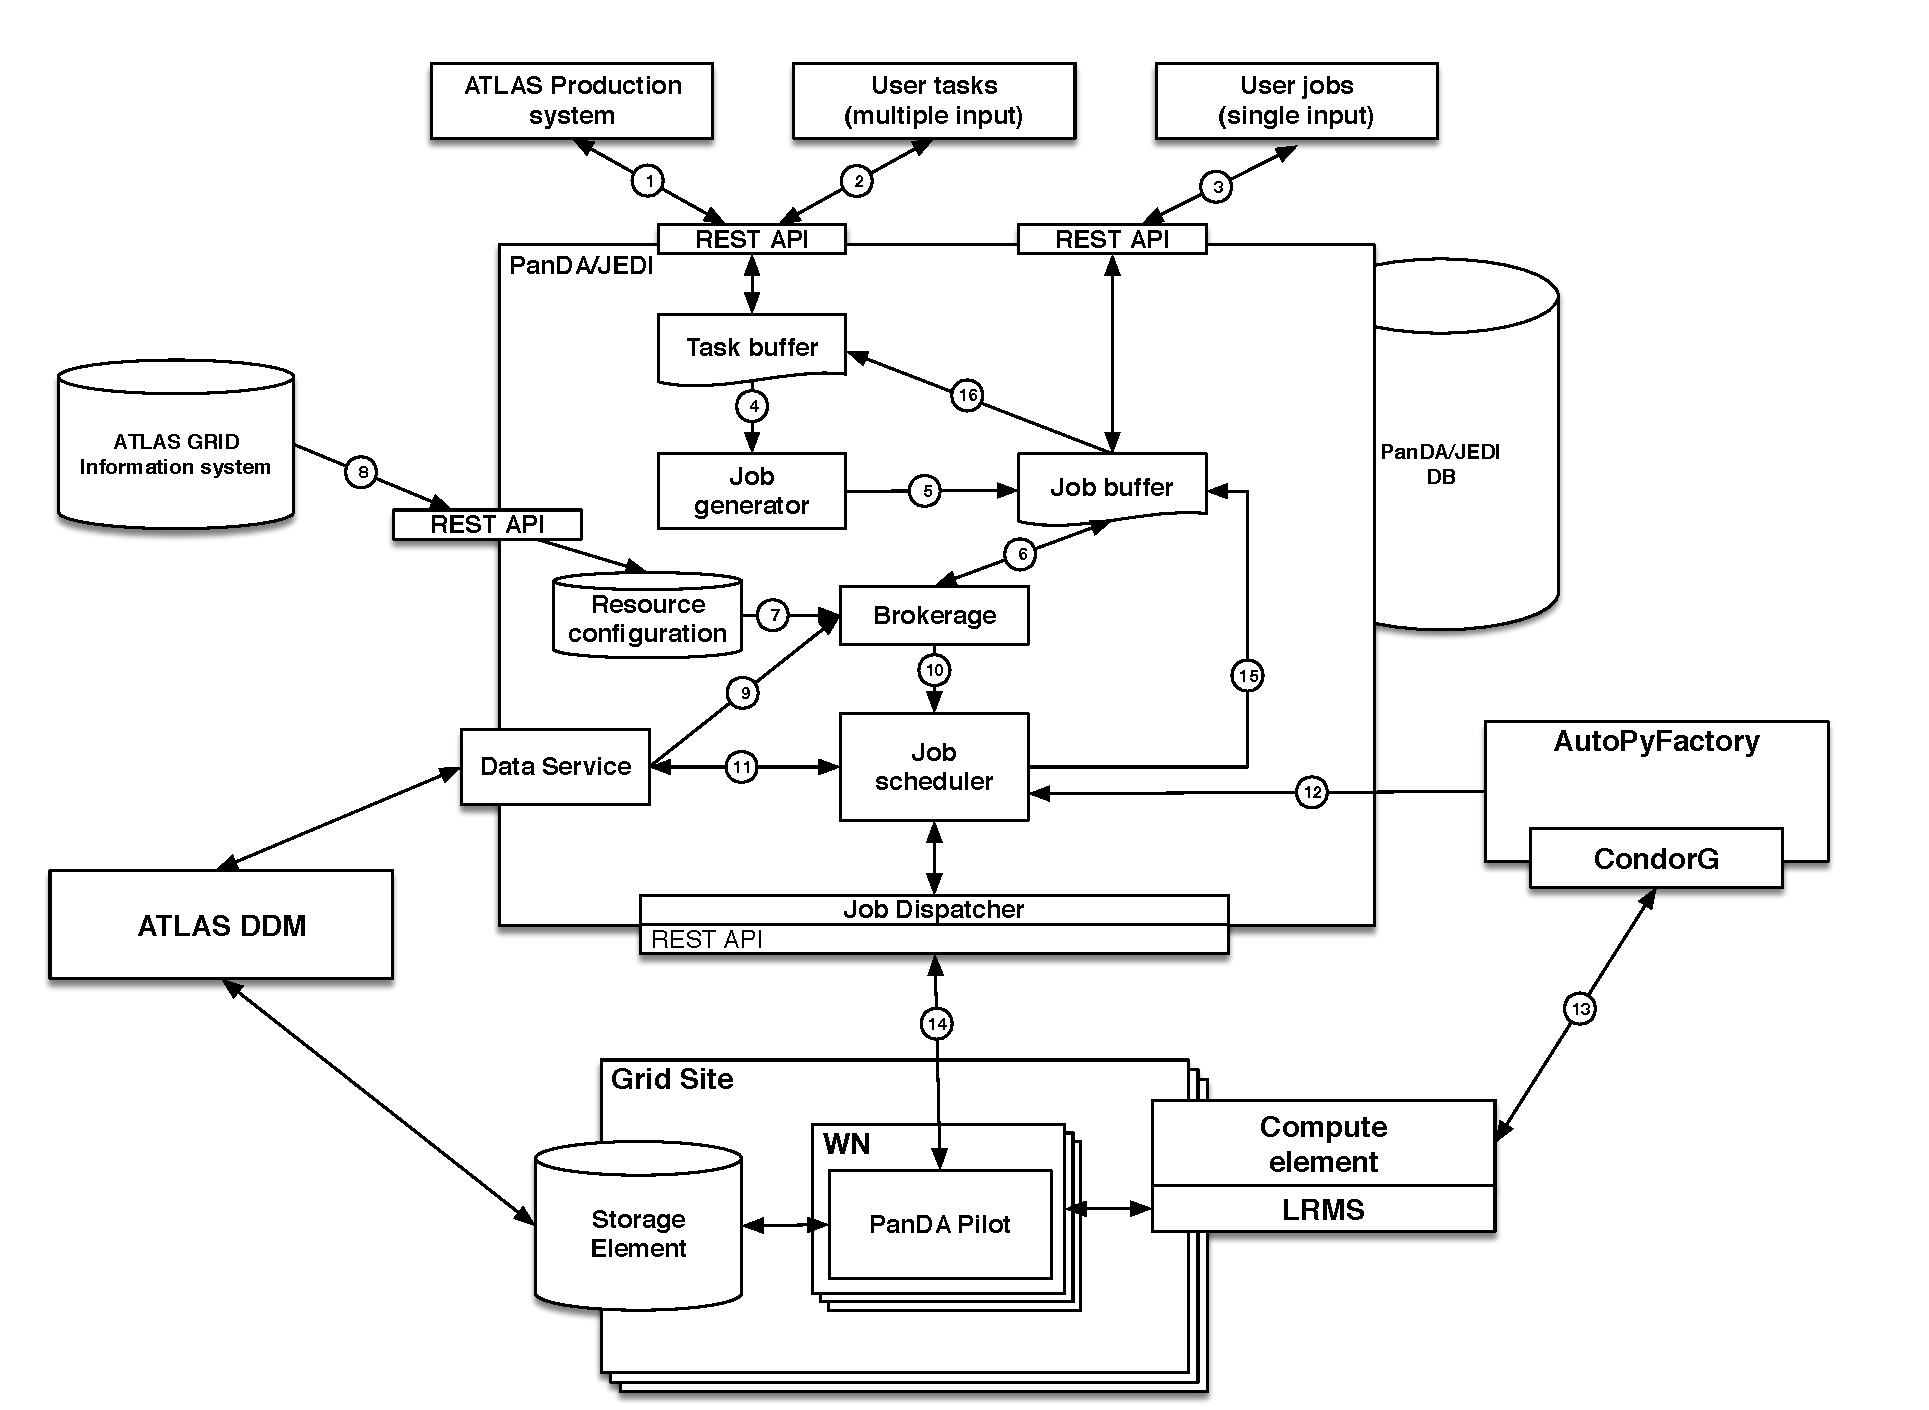
\includegraphics[width=0.75\textwidth]{images/PanDA_WMS.pdf}
  \caption{PanDA WMS architecture. Numbers indicate the JEDI-based execution
           process described in section~\ref{subsec:implementation}. Several
           subsystems, components, and architectural and communication details
           are abstracted to improve clarity.}
  \label{fig:architecture}
\end{figure*}

PanDA registers three types of workloads for execution: a set of tasks
submitted by the ATLAS Production system (Fig.~\ref{fig:architecture}:1); a
single user task submitted with a whole dataset
(Fig.~\ref{fig:architecture}:2); and a single job submitted by the user,
usually with a single input file (Fig.~\ref{fig:architecture}:3).

The Job Generator component renders a set of jobs from each registered task
based on the amount of input data and the amount of processed data per job by
taking into account the number of input files and number of events per job from
task parameters. Because jobs are not generated from a task all at once, the
job buffer is kept to a manageable size. This strategy enables the tuning of
task parameters based on initial job results and also task prioritization, if
needed (Fig.~\ref{fig:architecture}:4).

The Job Buffer component stores jobs that are waiting to be bound to a
specific resource for execution (Fig.~\ref{fig:architecture}:5). The Brokerage
component pulls jobs from the Job Buffer (Fig.~\ref{fig:architecture}:6),
binding each job to a compute resource based on job requirements, resource
capability (Fig.~\ref{fig:architecture}:7 and (Fig.~\ref{fig:architecture}:8),
and data availability (Fig.~\ref{fig:architecture}:9). Note that the Resource
Configuration component is also called Schedconfig.

The Job Scheduler component stores bound jobs that are waiting to be scheduled
on the assigned resource and executed (Fig.~\ref{fig:architecture}:10). Before
scheduling each job, the Job Scheduler checks whether input data are available
and, if needed, requests a transfer to the storage associated with the target
resource (Fig.~\ref{fig:architecture}:11).

Meanwhile, AutoPyFactory defines PanDA Pilots based on the number of jobs that
are bound and ready to execute, and it submits these pilots to a Condor-G agent
(Fig.~\ref{fig:architecture}:12). Condor-G schedules these pilots on the
required sites (Fig.~\ref{fig:architecture}:13). Once active, pilots interact
with the Job Dispatcher to pull jobs for execution
(Fig.~\ref{fig:architecture}:14). Depending on task and job parameters, failed
jobs may be rescheduled with a new job identifier
(Fig.~\ref{fig:architecture}:15).

Once all of a task's jobs have been executed and, depending on the failure
policy, all or most of the output data have been collected, a task is marked as
done. At that point, no more jobs will be generated for that task, and ATLAS
Production System or single users will be informed about the completion of the
task (Fig.~\ref{fig:architecture}:16). Tasks can also be marked as failed,
depending on whether a user-defined threshold for number of failures has been
exceeded.


% ---------------------------------------------------------------------------
\subsection{Job State Definitions in PanDA}
\label{subsec:jobstatedefs}

The life cycle of the job in the PanDA system is split into a series of
sequentially changing states. Each state is literally coupled with the PanDA
job status used by the different algorithms and monitoring. The status reflects
the current step of the job processing since the time that the job was
submitted to the system, transferred to the particular resource and finally
executed. Figure~\ref{fig:jobstates} illustrates the life cycle of jobs
submitted to PaNDA WMS.

% For two-column wide figures use
\begin{figure*}
% Use the relevant command to insert your figure file.
% For example, with the graphicx package use
  \includegraphics[width=0.75\textwidth]{images/job-state-diagram.png}
% figure caption is below the figure
\caption{This is a job state transitions model diagram for PanDA.}
\label{fig:jobstates}
\end{figure*}

Jobs are injected into the system as a ``job parameters'' object with a
``Pending'' status by JEDI in ATLAS or by the PanDA client otherwise.
Initially, this object is represented by a string containing unsorted
parameters. Next, the string is processed, the parameters of the job are sorted
into dedicated database fields, and the status is changed to ``Defined.'' After
that, the job is processed through the brokerage algorithm and assigned to a
particular resource using a PanDA queue, and the status is changed to
``Assigned''. Then, the status is changed to ``Waiting'' while the PanDA server
checks the availability of the input data and the required software at the
resource before changing the job's status to ``Activated''. An activated job is
a job which is ready to be dispatched to the next corresponding pilot. When the
job is dispatched and taken by the pilot, the job's status is changed to
``Sent''. At this time, the handling of the job processing has not been
delegated to the pilot yet, and thus, the next few job states correspond to the
steps of the job processing on the assigned resource. When the job status
changes to ``Starting'', the pilot is starting the job on a worker node or
local batch system, after which the status becomes ``Running'' when the job
begins running on a worker node. At this time, the progression of states is
once again handled by the server instead of by the pilot. After the job
finishes executing and output and log files are transferred, the PanDA server
is responsible for registering the files in the file catalog. At the same time,
the pilot returns the final status of the job to the server by communicating
that the job either succeeded or failed. During this process, the job has a
``Holding'' status. The PanDA server checks the output files regularly by using
cron, and it assigns the final ``Finished'' or ``Failed'' status to the job.
There are also some other statuses, the two most important of which are
``Cancelled'' for manually killed jobs and ``Closed'' for jobs which were
terminated by the system before completion so they could be reassigned to other
sites.

% ---------------------------------------------------------------------------
\subsection{Brokerage Characterization}
\label{subsec:brokerage}

The purpose of PanDA Broker is to assign a job to a queue corresponding to a
resource where the job will run. A job has parameters which constrain where it
can be assigned, and a queue has attributes which constrain what can be
assigned to it. This section details how PanDA Broker solves the constraint
problems and assigns jobs to queues, and it contains a benchmark study.

The general brokerage algorithm works in the following way. Given a set of jobs
and a set of queues, PanDA Broker checks each job's parameters, such as
requested nodes and requested wall time, against each queue's attributes, which
represent the allowable values for job parameters for the queue's underlying
resource. For each job, a set of candidate queues is generated from this
matching procedure, and then one queue is chosen according to a weighting
function which takes factors such as the resource's network bandwidth and
sharing policies into account.

Pseudo-code for the brokerage algorithm is shown as idealized Python code in
\ref{lst:list.py}. The \texttt{match\_constraints} function matches a job's
parameters $\{p_1, p_2, \ldots, p_m\}$ to a queue's attributes $\{a_1, a_2,
\ldots, a_n\}$, where $n \geq m$, in such a way that mapped parameters are
tested for membership in the set of allowed values specified in the attribute.
The \texttt{calculate\_weight} function used by ATLAS takes many factors into
account including current availability, network bandwidth, and sharing policies.

\lstinputlisting[language=Python, 
         label={lst:list.py}, 
         caption={Caption}]{list.py}

%-  vim:set syntax=tex:
